%%%%%%%%%%%%%%%%%%%%%%%%%%%%%%%%%%%%%%%%%%%%%%%%%%%%%%%%%%%%%%%%%%%%%%%%%%%%%%%
%                                                                             %
% VARIATIONAL MONTE CARLO METHODS FOR QUANTUM DOTS, by Matteo Seclì           %
%                                                                             %
% This eBook is meant to be used as the BSc Thesis of the author.             %
% The predicted date of the discussion is 22/07/2015 at the University of     %
% Trento.                                                                     %
%                                                                             %
% For licensing information, look at the LICENSE file shipped with this       %
% document.                                                                   %
%                                                                             %
% The original location of this project is at                                 %
% https://github.com/matteosecli/QMC.                                         %
%                                                                             %
% Title: Variational Monte Carlo Methods for quantum dots                     %
%                                                                             %
% Author: Matteo Seclì <secli.matteo@gmail.com>                               %
%                                                                             %
% Language: English                                                           %
%                                                                             %
% Character set encoding: UTF-8                                               %
%                                                                             %
% *** START OF THIS BACHELOR THESIS PROJECT ***                               %
%                                                                             %
%%%%%%%%%%%%%%%%%%%%%%%%%%%%%%%%%%%%%%%%%%%%%%%%%%%%%%%%%%%%%%%%%%%%%%%%%%%%%%%

%%%%%%%%%%%%%%%%%%%%%%%%%%%%%%%%%%%%%%%%%%%%%%%%%%%%%%%%%%%
% Definition of useful commands							  %
%%%%%%%%%%%%%%%%%%%%%%%%%%%%%%%%%%%%%%%%%%%%%%%%%%%%%%%%%%%
\newcommand{\ve}[1]{\mathbf{#1}}
\newcommand{\ham}{\mathcal{H}}
\newcommand{\ket}[1]{\left| #1 \right\rangle}
\newcommand{\bra}[1]{\left\langle #1 \right|}
\newcommand{\bracket}[2]{\left\langle #1 | #2 \right\rangle}
\newcommand{\bracketop}[3]{\left\langle #1 |#3| #2 \right\rangle}

%%%%%%%%%%%%%%%%%%%%%%%%%%%%%%%%%%%%%%%%%%%%%%%%%%%%%%%%%%%
% Basic class definitions, typesetting, bibliography      %
%%%%%%%%%%%%%%%%%%%%%%%%%%%%%%%%%%%%%%%%%%%%%%%%%%%%%%%%%%%
\documentclass[a4paper,twoside,11pt]{book}
\usepackage[utf8]{inputenc}
\usepackage{type1cm}
\usepackage{setspace}
\usepackage[english]{babel}
\usepackage{datetime}

\usepackage[backend=bibtex, sorting=none]{biblatex}
\addbibresource{bibliography.bib}

%%%%%%%%%%%%%%%%%%%%%%%%%%%%%%%%%%%%%%%%%%%%%%%%%%%%%%%%%%%
% Hyperref configuration                                  %
%%%%%%%%%%%%%%%%%%%%%%%%%%%%%%%%%%%%%%%%%%%%%%%%%%%%%%%%%%%
\usepackage[%hypertex,
	unicode=true,
	plainpages = false, 
	pdfpagelabels, 
	bookmarks=true,
	bookmarksnumbered=true,
    bookmarksopen=true,
	breaklinks=true,
	backref=false,
	colorlinks=true,
	linkcolor = blue,		% Use "blue" if you want to highlight them
	urlcolor  = blue,
	citecolor = red,
	anchorcolor = green,
	hyperindex = true,
	linktocpage = true,
	hyperfigures
]{hyperref}


%%%%%%%%%%%%%%%%%%%%%%%%%%%%%%%%%%%%%%%%%%%%%%%%%%%%%%%%%%%
% Grahpics                                                %
%%%%%%%%%%%%%%%%%%%%%%%%%%%%%%%%%%%%%%%%%%%%%%%%%%%%%%%%%%%
\usepackage{graphicx}
\usepackage{xcolor}
\graphicspath{{figures/PNG/}{figures/PDF/}{figures/}}
\usepackage{tikz}
\usepackage[siunitx]{circuitikz}


%%%%%%%%%%%%%%%%%%%%%%%%%%%%%%%%%%%%%%%%%%%%%%%%%%%%%%%%%%%
% Standard environments                                   %
%%%%%%%%%%%%%%%%%%%%%%%%%%%%%%%%%%%%%%%%%%%%%%%%%%%%%%%%%%%
\usepackage{float}
\usepackage[font={small,it}]{caption}[2013/01/06] % Minimum version required for incompatibility with breqn
\usepackage{subcaption}
\usepackage{listingsutf8}
\usepackage{enumitem}


%%%%%%%%%%%%%%%%%%%%%%%%%%%%%%%%%%%%%%%%%%%%%%%%%%%%%%%%%%%
% Math                                                    %
%%%%%%%%%%%%%%%%%%%%%%%%%%%%%%%%%%%%%%%%%%%%%%%%%%%%%%%%%%%
\usepackage{amsmath}
\usepackage{amssymb}	
\usepackage{amsthm}
\usepackage{cancel}
\usepackage{braket}
\usepackage{siunitx}
\DeclareSIUnit\atomicunit{a.u.}
\usepackage{breqn}
\usepackage{geometry}
\renewenvironment{proof}{\vskip 1em \noindent\textsc{Proof:}}{\begin{flushright}$\blacksquare$\end{flushright}\vskip 1em}


%%%%%%%%%%%%%%%%%%%%%%%%%%%%%%%%%%%%%%%%%%%%%%%%%%%%%%%%%%%
% datetime specific configuration                         %
%%%%%%%%%%%%%%%%%%%%%%%%%%%%%%%%%%%%%%%%%%%%%%%%%%%%%%%%%%%
\newdateformat{monthyear}{\monthname[\THEMONTH] \THEYEAR}


%%%%%%%%%%%%%%%%%%%%%%%%%%%%%%%%%%%%%%%%%%%%%%%%%%%%%%%%%%%
% TikZ specific configuration                             %
%%%%%%%%%%%%%%%%%%%%%%%%%%%%%%%%%%%%%%%%%%%%%%%%%%%%%%%%%%%
\usetikzlibrary{shapes.geometric, arrows, patterns}
\tikzstyle{startstop} = [rectangle, rounded corners, minimum width=3cm, minimum height=1cm,text centered, draw=black, fill=red!30]
\tikzstyle{io} = [trapezium, trapezium left angle=70, trapezium right angle=110, minimum width=3cm, minimum height=1cm, text centered, draw=black, fill=blue!30]
\tikzstyle{process} = [rectangle, minimum width=3cm, minimum height=1cm, text centered, text width=3cm, draw=black, fill=orange!30]
\tikzstyle{decision} = [diamond, minimum width=3cm, minimum height=1cm, text centered, draw=black, fill=green!30]
\tikzstyle{arrow} = [thick,->,>=stealth]


%%%%%%%%%%%%%%%%%%%%%%%%%%%%%%%%%%%%%%%%%%%%%%%%%%%%%%%%%%%
% xcolor specific configuration                           %
%%%%%%%%%%%%%%%%%%%%%%%%%%%%%%%%%%%%%%%%%%%%%%%%%%%%%%%%%%%
\definecolor{dkgreen}{rgb}{0,0.6,0}
\definecolor{dred}{rgb}{0.545,0,0}
\definecolor{dblue}{rgb}{0,0,0.545}
\definecolor{lgrey}{rgb}{0.9,0.9,0.9}
\definecolor{gray}{rgb}{0.4,0.4,0.4}
\definecolor{darkblue}{rgb}{0.0,0.0,0.6}


%%%%%%%%%%%%%%%%%%%%%%%%%%%%%%%%%%%%%%%%%%%%%%%%%%%%%%%%%%%
% ListingsUTF8 specific configuration                     %
%%%%%%%%%%%%%%%%%%%%%%%%%%%%%%%%%%%%%%%%%%%%%%%%%%%%%%%%%%%
\lstdefinelanguage{cpp}{
	backgroundcolor=\color{lgrey},  
	basicstyle=\footnotesize \ttfamily \color{black} \bfseries,   
	breakatwhitespace=false,       
	breaklines=true,               
	captionpos=b,                   
	commentstyle=\color{dkgreen},   
	deletekeywords={...},          
	escapeinside={\%*}{*)},                  
	frame=single,                  
	language=C++,                
	keywordstyle=\color{purple},  
	morekeywords={BRIEFDescriptorConfig,string,TiXmlNode,DetectorDescriptorConfigContainer,
		istringstream,cerr,exit}, 
	identifierstyle=\color{black},
	stringstyle=\color{blue},      
	numbers=right,                 
	numbersep=5pt,                  
	numberstyle=\tiny\color{black}, 
	rulecolor=\color{black},        
	showspaces=false,               
	showstringspaces=false,        
	showtabs=false,                
	stepnumber=1,                   
	tabsize=5,                     
	title=\lstname,                 
}


%%%%%%%%%%%%%%%%%%%%%%%%%%%%%%%%%%%%%%%%%%%%%%%%%%%%%%%%%%%
% Some black magic                                        %
%%%%%%%%%%%%%%%%%%%%%%%%%%%%%%%%%%%%%%%%%%%%%%%%%%%%%%%%%%%
%\makeatletter
%	\renewcommand{\bibsection}{\chapter{\bibname}}
%\makeatother


%%%%%%%%%%%%%%%%%%%%%%%%%%%%%%%%%%%%%%%%%%%%%%%%%%%%%%%%%%%
% Metadata                                                %
%%%%%%%%%%%%%%%%%%%%%%%%%%%%%%%%%%%%%%%%%%%%%%%%%%%%%%%%%%%
\def\THauthor{Matteo Zortea}
\def\THsupervisor{Raffaello Potestio}
\def\THtitle{Physics at negative absolute temperature} % title
\def\THdate{\monthyear\today}
\def\THplace{Trento}
\title{\THtitle}
\author{\THauthor}


%%%%%%%%%%%%%%%%%%%%%%%%%%%%%%%%%%%%%%%%%%%%%%%%%%%%%%%%%%%
% Actual text                                             %
%%%%%%%%%%%%%%%%%%%%%%%%%%%%%%%%%%%%%%%%%%%%%%%%%%%%%%%%%%%

\begin{document}

\frontmatter
%%%%%%%%%%%%%%%%%%%%%%%%%%%%%%%%%%%%%%%%%%%%%%%%%%%%%%%%%%%
%                                                         %
% TITLEPAGE                                               %
%                                                         %
%                                                         %
% This file is part of a BSc Thesis Project. See the      %
% LICENSE file for more information about licensing.      %
%                                                         %
% Author:     Matteo Seclì <secli.matteo@gmail.com>       %
% A.Y.:       2014/2015                                   %
% URL:        https://github.com/matteosecli/QMC          %
%                                                         %
%%%%%%%%%%%%%%%%%%%%%%%%%%%%%%%%%%%%%%%%%%%%%%%%%%%%%%%%%%%

\graphicspath{{Frontmatter/figures/PNG/}{Frontmatter/figures/PDF/}{Frontmatter/figures/}}

\begin{titlepage}
	\newgeometry{margin=3.5cm}
	
	\begin{center}
	
		% Logo
		
\includegraphics[scale=0.12]{logo_unitn}\\[0.4cm]
			
		\vspace{0.8cm}
		
		{ \Huge \scshape University of Trento }\\[0.25cm]
		{ \Large \scshape Department of Physics }\\[2cm]

		{ \Large \scshape Thesis }\\[0.05cm]
		{ \itshape for the degree in }\\[0.05cm]
		{ \Large \scshape Bachelor of Science }\\[2cm]
		
		
		% Title
		{ \huge \bfseries \THtitle }
		
		\vfill
				
		% Author and supervisor
		\begin{minipage}[t]{0.45\textwidth}
			\begin{flushleft} %\large
				{ \large \scshape Supervisor: } \\[0.25cm]
				{ Prof. \THsupervisor }\\[0.10cm]
			\end{flushleft}
		\end{minipage}
		\begin{minipage}[t]{0.45\textwidth}
			\begin{flushright} %\large
				{ \large \scshape Candidate: }\\[0.25cm]
				{ \THauthor }
			\end{flushright}
		\end{minipage}
		
		\vspace{2cm}
		
		% Bottom of the page
		{\large \scshape Academic Year 2020/2021}
		
	\end{center}
	
	\restoregeometry
\end{titlepage}
%\onehalfspacing	% Set 1.5 lines spacing for better readability
%%%%%%%%%%%%%%%%%%%%%%%%%%%%%%%%%%%%%%%%%%%%%%%%%%%%%%%%%%%
%                                                         %
% PREFACE                                                 %
%                                                         %
% This file is part of a BSc Thesis Project. See the      %
% LICENSE file for more information about licensing.      %
%                                                         %
% Author:     Matteo Seclì <secli.matteo@gmail.com>       %
% A.Y.:       2014/2015                                   %
% URL:        https://github.com/matteosecli/QMC          %
%                                                         %
%%%%%%%%%%%%%%%%%%%%%%%%%%%%%%%%%%%%%%%%%%%%%%%%%%%%%%%%%%%

\chapter{Preface}
Motivazioni e ringraziamenti
\begin{flushright}
	{ \THauthor }
\end{flushright}
\begin{flushleft}
	{ \THplace, \THdate }
\end{flushleft}



%%%%%%%%%%%%%%%%%%%%%%%%%%%%%%%%%%%%%%%%%%%%%%%%%%%%%%%%%%%
%                                                         %
% CHAPTER 01:                                             %
% What are quantum dots?                                  %
%                                                         %
% This file is part of a BSc Thesis Project. See the      %
% LICENSE file for more information about licensing.      %
%                                                         %
% Author:     Matteo Seclì <secli.matteo@gmail.com>       %
% A.Y.:       2014/2015                                   %
% URL:        https://github.com/matteosecli/QMC          %
%                                                         %
%%%%%%%%%%%%%%%%%%%%%%%%%%%%%%%%%%%%%%%%%%%%%%%%%%%%%%%%%%%

\chapter{Introduction}

Everyone has an intuitive idea of what temperature is in everyday life: it is a quantity that tells us how \emph{hot} or \emph{cold} an object is. \\
Temperature is an intensive property of a system, which means that it does not depend on the object's dimensions nor on the quantity of matter contained in it. \\
Temperature is measured via thermometers and, since it is a physical quantity, it must be exressed in terms of physical units. All thermometers are expected to give the same number when used to measure the temperature of the same object, provided that 
the number is expressed always in the same physical unit. This can be possible if the thermometers are accurately calibrated according to some critera that make the calibration process reproducible. 
A roughly good calibration of a thermometer in the so called Celsius scale can be done by assigning the instrument a value of $0^\circ$C (0 degrees Celsius) at the freezing point of water, and $100^\circ$C at the boiling point of water. A more sophisticated and precise way to calibrate a thermometer 
on the Celsius scale consists in assigning the value of $-273.15^\circ$C to the \emph{coldest} temperature admitted according to nowadays' physics, and $0.01^\circ$ C to the triple point of water, that 
is the point in which water coexists in liquid, solid and gaseous form. One can then extract a measure of all the other values of temperature by assuming a linear relation between temperature and the property in the material used as a thermometer,
such as an elastic deformation. \\
Another interesting temperature scale is the one measured in Kelvin (K), called the \emph{absolute temperature}. This scale of temperature is 
defined in a way such that it gives a values of $0$ K at the coldest possible situation admitted by physics, the so called \emph{absolute zero} point: this means that no physical systems can be cooled more than a system 
whose absolute temperature is $0$ K. \par
\vspace{10pt}
The purpose of this thesis is to introduce the concept of \emph{negative absolute temperatures}. This does not constitute a contradiction to what told before because negative absolute temperatures should not be searched below the absolute zero, but rather 
above infinity: negative absolute temperatures are hotter than all the positive ones. The world of negative absolute temperatures is often accompanied by strange phenomena: for example, when a system at negative temperature is put into contact with one at positive temperature, the former gives heat to the latter,
leading the temperature of the former to be lowered and the temperature of the latter to be raised. \par
\vspace{10pt}
In the first chapter of this thesis I will introduce the concept of temperature in a rigorous way according to physical laws, justifying the existence of negative absolute temperatures basing on thermodynamical arguments. \\
A simple system that admits negative temperatures, namely the two level system, will then be presented in chapter \ref{ch:TLS}. \\
In chapter \ref{ch:PandP} I will show that negative absolute temperatures were experimentally observed by Purcell and Pound in 1950. 
After that discovery, some criticisms were moved against the definition of the entropy used to define the absolute scale, putting in doubt the existence of negative temperatures: this will be discussed in chapter \ref{ch:entropy}. \\
Finally some simulations of a systems at negative temperature will be presented in the last chapter.

\tableofcontents

\mainmatter
\subsubsection*{Temperature as an equilibrium property}
Temperature can be more sistematically defined starting from the concept of \emph{equilibrium}. We consider a thermodynamic system to be in equilibrium when 
no changes are observed in any macroscopic observable and when the system does not exchange heat nor work with the environment. In particular we say that the system is at \emph{thermal equilibrium} when no heat is exchanged by the system, and
at \emph{mechanical equilibirum} when no work is done by or on the system. \\
Let us consider three systems $A, B, C$ whose equilibrium properties are described by the variables
$\{X_1, X_2, \dots\}$, $\{Y_1, Y_2, \dots\}$ and $\{Z_1, Z_2, \dots\}$. \\
If $A$ and $B$ are in equilibrium for some values $\{X_1, X_2, \dots\}$ and $\{Y_1, Y_2, \dots\}$ of the coordinates, then there must be a relation between $\{X_1, X_2, \dots\}$ and $\{Y_1, Y_2, \dots\}$ which can be expressed as
\begin{equation*}
    f_{AB}(X_1, X_2, \dots, Y_1, Y_2, \dots) = 0
\end{equation*}
In an analogous manner, if $B$ and $C$ are in equilibrium for some values $\{Y_1', Y_2', \dots\}$ and $\{Z_1, Z_2, \dots\}$ of the coordinates, then there must be a constrain on the values $\{Y_1', Y_2', \dots\}$ and $\{Z_1, Z_2, \dots\}$, which we express as
\begin{equation*}
    f_{BC}(Y_1', Y_2', \dots, Z_1, Z_2, \dots) = 0
\end{equation*}
The equations above can be inverted to espress one thermodynamic coordinate as a function of the others, or in other words, the above expressions may be written as
\begin{gather*}
    Y_1 = g_{AB} (X_1, X_2, \dots, Y_2, \dots) \\
    Y_1' = g_{BC} (Y_2', \dots, Z_1, Z_2, \dots)
\end{gather*}
Now let us bring the system $B$ in the same state in both cases, which means imposing $Y_1 = Y_1'$ and $Y_2 = Y_2'$. The last two equations implies that 
\begin{equation}
    g_{AB} (X_1, X_2, \dots, Y_2, \dots) = g_{BC} (Y_2, \dots, Z_1, Z_2, \dots)
    \label{eq:equality_of_g}
\end{equation}
or
\begin{equation*}
    G_{ABC} (X_1, X_2, \dots, Y_2, \dots, Z_1, Z_2, \dots) = 0
\end{equation*}
One can use this relation to express $X_1$ as 
\begin{equation}
    X_1 = h_{ABC}(X_2, \dots, Y_2, \dots, Z_1, Z_2)
    \label{eq:X1_equilibrium_ABC}
\end{equation}
According to the zeroth principle of thermodynamics, which states that if $A$ and $B$ are in equilibrium and $B$ and $C$ are in equilibrium then $A$ and $C$ are in equilibrium 
\footnote{or, alternatively, that equilibrium is an equivalence relation}, then
there must be a constrain on the values ${X_1, X_2, \dots}$, ${Z_1, Z_2, \dots}$ which can be expressed as 
\begin{equation*}
    f_{AC} (X_1, X_2, \dots, Z_1, Z_2, \dots) = 0
\end{equation*}
which means that $X_1$ can be expressed as
\begin{equation}
    X_1 = g_{AC} (X_2, \dots, Z_1, Z_2, \dots)
    \label{eq:X1_equilibrium_AC}
\end{equation}
imposing the equality between \ref{eq:X1_equilibrium_ABC} and \ref{eq:X1_equilibrium_AC}
\begin{equation*}
    g_{AC} (X_2, \dots, Z_1, Z_2, \dots) = h_{ABC}(X_2, \dots, Y_2, \dots, Z_1, Z_2)
\end{equation*}
The term on the lefts does not depend on the coordinates of $B$. This means that both $g$ functions in equation \ref{eq:equality_of_g} must be of the type
\begin{gather*}
    g_{AB}(X_1, X_2, \dots, Y_2, \dots) = \Theta(X_1, X_2, \dots) + \phi(Y_2, \dots) \\
    g_{BC}(Y_2, \dots, Z_1, Z_2, \dots) = \Theta(Z_1, Z_2, \dots) + \phi(Y_2, \dots)
\end{gather*}
so that the dependence on $\{Y\}$ gets cancelled out when equating the two functions leading to 
\begin{equation*}
    \Theta_A(X_1, X_2, \dots) = \Theta_B(Y_1, Y_2, \dots)
\end{equation*}
We started this reasoning by assuming equilibrium between $A-B$ and $B-C$, but one could repeat this reasoning by assuming
equilibrium between $A-C$ and $B-C$ obtaining the same result in terms of $\{Z_1, Z_2, \dots\}$. But also, because of the properties of the equivalence relation,
one can extend the reasoning to an arbitrary number of systems. This means that if $N$ systems are in equilibrium, then there must be a function $\Theta$ such that
\begin{equation*}
    \Theta_A(X_1, X_2, \dots) = \Theta_B(Y_1, Y_2, \dots) = \Theta_C(Z_1, Z_2, \dots) = \dots
\end{equation*}
Let us call this function \emph{empirical temperature}, and its value on a set of coordinates identifies a particular equivalence class of systems at equilibrium. \\
What just proven shows that systems at equilibrium are identified by the same value of a certain function $\Theta$. By the way no specifications are given about the origin 
of this function and which precise value it has for a given set of systems at equilibrium. In fact there are multiple ways to define the values of such function, leading
to many \emph{temperature scales}. \\
An example of a possible way to define a scale of temperature is the one that concerns ideal gases. Practically it consists in assigning a value $\Theta = 273.16$ degrees Kelvin (K) at the triple point of water (coexistence of ice-water-gas) and then
other values of temperature for ideal gases are defined via the relation 
\begin{equation*}
    T(K) = \lim_{P \to 0} 273.16 \times \frac{(PV)_{system}}{(PV)_{ice-water-gas}}
\end{equation*}
because for an ideal gas $T \propto PV$. \\
Another possible definition of the function $\Theta$, the one relevant for what follows, will be presented later in this chapter.

\subsubsection*{Thermodynamic temperature}
Once introducing an entropy as a function of the energy $S(E)$ it is possible to define a so called \emph{thermodynamic temperature} via the relation $\frac{1}{T} = \frac{\partial S}{\partial E}$.
To see why this makes sense it is convenient to look at this example. \\
First let us consider a system isolated from the environment, so that it cannot exchange heat or work (energy fixed). Let us indicate a generical
state of the system by the microscopic coordinates $\ve{x} = (q_1, \dots, q_n, p_1, \dots, p_n)$ where $(q_i, p_i)$ is a pair of canonical coordinates. If $\ham(\ve{x})$ denotes the hamiltonian of the system,
the condition
\begin{equation}
    \ham(\ve{x}) = E
    \label{eq:microcanonical_condition}
\end{equation}    
for a certain value of energy $E$, defines a microcanonical ensemble. \\
The central postulate of a priori probability in statistical mechanics states that all the microstates satisfying \ref{eq:microcanonical_condition} are equally probable. In other words, one can
define a probability density function
\begin{equation*}
    p(E, \ve x) = \frac{1}{\Omega(E, \ve x)} \ \delta(H(\ve x) - E)
\end{equation*}
where $\Omega(E, \ve x)$ denotes the volume of the phase space satisfying equation \ref{eq:microcanonical_condition}. \\
We also assume the Boltzmann definition of entropy \footnote{This assumption is non trivial and will be deeply discussed in section SECTION}
\begin{equation}
    S(E, \ve x) = k_B \log(\Omega(E, \ve x))
    \label{eq:Boltzmann_entropy}
\end{equation}
Let us now consider two systems with fixed energies $E_1$, $E_2$ when separated. By putting them into contact and allowing them exchanging energy, one can create another system 
with fixed energy $E = E_1 + E_2$ which can be studied in the microcanonical ensemble.
For fixed values $E_1$ and $E_2 = E - E_1$ the phase space volume allowed for the system is 
\begin{equation*} 
    \Omega_{E_1}(E, \ve x) = \Omega_1(E_1, \ve x_1) \cdot \Omega_2(E_2, \ve x_2)
\end{equation*}
but $E_1$ (and as a consequence $E_2 = E - E_1$) is free to move between $0$ and $E$, hence the total phase space volume is given by an integral sum of the volumes at fixed $E_1$ \\
\begin{gather*}
    \Omega(E, \ve x) = \int_0^E \, dE_1 \int_0^E \, dE_2 \ \Omega_1(E_1, \ve x_1) \ \Omega_2(E_2, \ve x_2) \ \delta(E_1 + E_2 - E) = \\
    = \int_0^E \, dE_1 \ \Omega_1(E_1, \ve x_1) \ \Omega_2(E - E_1, \ve x_2)
\end{gather*}
By using now equation \ref{eq:Boltzmann_entropy} the last equation can be written as 
\begin{equation*}
    \Omega(E, \ve x) = \int_0^E \, dE_1 \ e^{(S_1(E_1) + S_2(E-E_1))/k_B}
\end{equation*}
In the limit $N \to +\infty$ the integral becomes sharply peaked around a value $E_1^*$ and it can be evaluated using the Laplace's method
\begin{equation*}
    \Omega(E, \ve x) \approx C e^{(S_1(E_1^*) + S_2(E-E_1^*))/k_B}
\end{equation*}
The energy value that maximes $\Omega(E, \ve x)$ is the one that is represented by the largest number of microstates, hence the most probable or, in other words, the one that it is most likely at equilibrium. This value corresponds to the maximum of the exponential factor $S_1(E_1^*) + S_2(E-E_1^*)$ and can then be found as 
\begin{equation*}
    0 = \frac{\partial}{\partial E_1}(S_1(E_1) + S_2(E-E_1)) = \frac{\partial S_1(E_1)}{\partial E_1} - \frac{\partial S_2(E_2)}{\partial E_2} 
\end{equation*}
or
\begin{equation*}
    \frac{\partial S_1(E_1)}{\partial E_1} = \frac{\partial S_2(E_2)}{\partial E_2} 
\end{equation*}
Hence any two systems at equilibrium satisfies this last equation. For what told in section (ADD SECTION REFERENCE), the function 
$\frac{\partial S}{\partial E}$ must be an empirical temperature or, better, because of dimensional arguments, an inverse of a temperature. Hence the condition can be read as 
\begin{equation*}
    T_1 = T_2
\end{equation*}
This justifies the definition given at the beginning of this section 
\begin{equation}
    \frac{1}{T} = \frac{\partial S(E)}{\partial E}
    \label{eq:absolute_temperature}
\end{equation}
The derivation of the last equation made use only of the zeroth principle of thermodynamics and physical consideration about equilibrium: in this sense the temperature defined via \ref{eq:absolute_temperature} sometimes is also called \emph{absolute temperature}. \\
A rather counterintuitive result at negative absolute temperatures concerns the direction of heat flow. Consider two systems $\mathcal{S}_1$ and $\mathcal{S}_2$ isolated and individually in thermal equilibrium at temperatures $T_1$ and $T_2$ respectively. We say that $\mathcal{S}_1$ is \textit{hotter} and $\mathcal{S}_2$ is \textit{colder} if, when 
$\mathcal{S}_1$ and $\mathcal{S}_2$ are put into contact, the heat flows from $\mathcal{S}_1$ to $\mathcal{S}_2$, and viceversa. When $\mathcal{S}_1$ and $\mathcal{S}_2$ are put into contact the change in $\mathcal{S}_1$'s entropy is $\delta S_1 = \frac{\delta Q}{T_1}$ and in $\mathcal{S}_2$'s is $\delta S_2 = -\frac{\delta Q}{T_2}$. If the process happens keeping 
the system $\mathcal{S} = \mathcal{S}_1 + \mathcal{S}_2$ thermally isolated from the environment, then we know that $\delta S = \delta S_1 + \delta S_2 > 0$ because of the second law of thermodynamics, which implies 
\begin{equation*}
    \delta Q \ \left(\frac{1}{T_1} - \frac{1}{T2}\right) > 0
\end{equation*}
One can now note that
\begin{enumerate}
    \item If $T_1, T_2 > 0$ and $T_1 > T_2$ then it must be $\delta Q < 0$
    \item If $T_1, T_2 < 0$ and $T_1 > T_2$ then it must be $\delta Q > 0$
    \item If $T_1 > 0$ and $T_2 < 0$ then it must be $\delta Q > 0$
\end{enumerate}
According to the convention that $\delta Q > 0$ means that the system absorbs a heat $\delta Q$, condition $1)$ means that heat flows from the system at negative temperature to the one at positive temperature or, in other words, that
systems at negative temperatures are hotter than those at positive ones. Instead, condition $2)$ means that when two systems at negative temperatures are put into contact, the system at lower temperature gives heat to the one at higher temperature. If one would make
a hierarchy of "hotness" of systems depending on the temperature, it would be 
\begin{equation*}
    0^+ < +\infty < -\infty < 0^-
\end{equation*}
This fact will be further explored in \hyperref[sec:TLS]{section 3}.

\subsubsection*{Intuitive interpretation of thermodynamic temperature}
Here I want to provide an insight into the meaning of the formal definition $\frac{1}{T} = \frac{\partial S(E)}{\partial E}$. According to this definition, the temperature is 
a measure of the tendency of a system to increase/decrease entropy when an amount of energy is added. When the temperature is positive, adding energy to the system always 
increases the entropy of the system, giving it access to more states. A negative temperature, on the other side, symbolizes the fact that the system decreases its entropy when an amout of energy is added: in other 
words this means that the number of accessible states for the system decreases as the energy increases. One can imagine that if the maximum energy state of a system is realised only by one or few microstates, the systems might admit a decreasing 
entropy as a function of energy, hence admitting negative temperatures. This idea will be formalized in the the \emph{Ramsey}'s criteria which provide the conditions under which a system admits negative temperature.
\chapter{Two levels system}
\label{ch:TLS}

\section{Two-levels systems admit negative temperatures}
The simplest system that can exhibit negative temperatures is the two levels system (TLS). \\
A TLS is a system, for example a particle, for which only two values of energy are admitted, say $E_1$ and $E_2$. Let us denote the 
corresponding eigenstates by $\ket{1}$ and $\ket{2}$. An example of such a system, which we may consider in the following derivations, can be a spin-$1/2$ fermion in a uniform magnetic field.
Let us now consider a system composed of $N$ TLS. It is convenient to introduce the occupation numbers $n_1, n_2$ which denote,
respectively, the number of TLS at energy $E_1$ and $E_2$. If we set $E_1=\epsilon$ and $E_2=0$ for simplicity, the energy of the system is
\begin{equation}
    E = n_1 E_1 + n_2 E_2 = n_1\epsilon
    \label{eq:TLS_ensemble_energy}
\end{equation}
where $n_1 + n_2 = N$. \\
One macrostate of the system is thus identified by its energy and the total number of particles. The number of microstates corresponding 
to one given macrostate is the number of ways in which one can rearrange the particles in a way such that the total energy remains fixed, that is 
\begin{equation*}
    \Omega(E, N) = \frac{N!}{n_1!n_2!} = \frac{N!}{n_1! \, (N-n_1)!}
\end{equation*}
which corresponds to the Boltzmann entropy 
\begin{equation}
    S(E, N) = k_B\ln\left(\frac{N!}{n_1! \, (N-n_1)!}\right)
    \label{eq:TLS_entropy_N}
\end{equation}
In the limit of large $N$ the last expression can be expanded by using the Stirling's formula $\ln(N!) \approx N\ln N - N$ which yields 
\begin{equation}
    S(E, N) \approx N \ln \left(\frac{N}{N-n_1}\right) + n_1 \ln\left(\frac{N-n_1}{n_1}\right)
    \label{eq:TLS_entropy_N_approx}
\end{equation}
By using relation \ref{eq:TLS_ensemble_energy}
\begin{equation}\begin{gathered}
    \frac{1}{T} = \frac{\partial S}{\partial E} = \frac{\partial S}{\partial n_1} \, \frac{\partial n_1}{\partial E} =
    \frac{k_B}{\epsilon} \, \ln\left(\frac{N - n_1}{n_1}\right) = -\frac{k_B}{\epsilon} \, \ln\left(\frac{E}{N\epsilon - E}\right)
\end{gathered} 
\label{eq:T_tls} 
\end{equation}
where in the last step I used equation \ref{eq:TLS_ensemble_energy} again inside the logarithm's argument. \\
A plot of the temperature as a function of the system's energy is reported in figure \ref{fig:temperature_TLS}. Negative temperatures occur in the region in which $E > \frac{N\epsilon}{2}$, which corresponds to the states in which there are more particles 
in the excited state than in the lower one. As mentioned at the end of chapter \ref{ch:temperature}, negative temperatures occur above $+\infty$ rather than below the absolute zero. When a TLS is cooled down to $\SI{0}{\degree\kelvin}$ all the spins lie in the ground state, i.e. the state of minimum energy.
As soon as one adds energy to the system, the temperature starts increasing and more and more particles get excited to the higher energy state untill the point in which, on average, we expect the particles to be half excited and half in the ground state, that is we have the same probability 
of having an excited particle or a particle in the ground state. This happens when the temperature is ideally infinite, either positive or negative, and this constitutes the state of maximum entropy. By keeping adding energy to the system one ends up having more particles in the excited state rather than in the lower one,
experiencing the \emph{population inversion}. \\
\begin{figure}[h]
    \centering 
    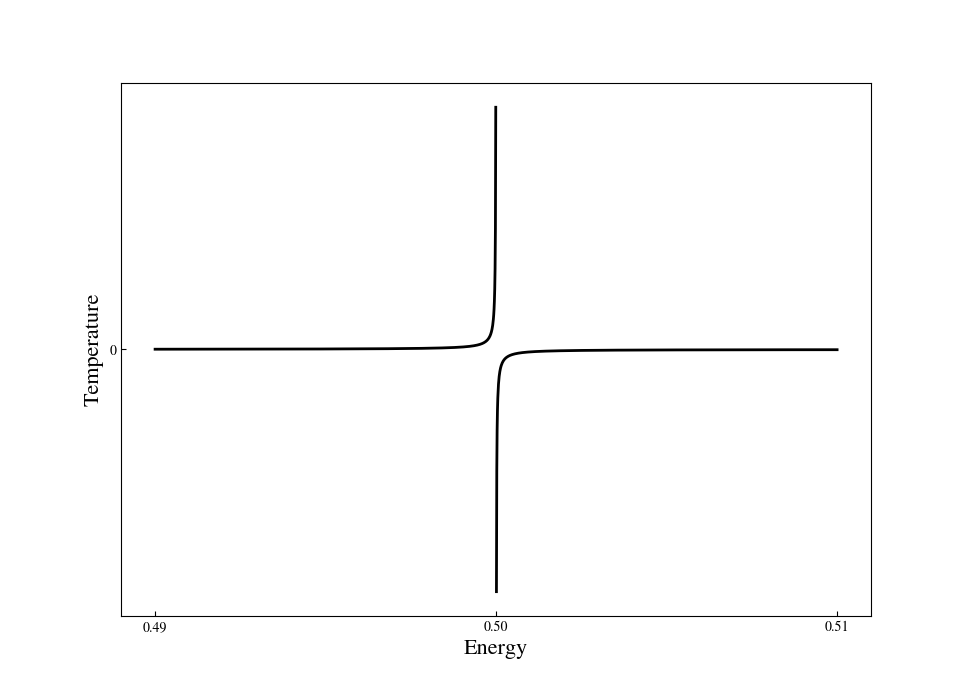
\includegraphics[scale=0.65]{images/temperature_TLS.png}
    \caption{The plot reports the temperature as a function of the energy ($E/N\epsilon$) in a two-levels system. When there are more excited particles than those in the lower state (energy $> 0.5$), the system exhibits negative absolute temperatures.}
    \label{fig:temperature_TLS}
\end{figure}
Equation \ref{eq:T_tls} can be rewritten as
\begin{equation*}
    \frac{1}{T} = \frac{k_B}{\epsilon} \ln\left(\frac{n_2}{n_1}\right)
\end{equation*}
which leads to 
\begin{equation}
    \frac{n_2}{n_1} = e^{-\epsilon/k_BT}
    \label{eq:spin_temperature}
\end{equation}
This formula allows us to introduce the so called \emph{spin temperature}. \\
In the derivation of the results for the two level system we implicitly assume that the spin system is
isolated from the environment and that the spins do not interact each other or, in other words, that each spin is isolated from the rest of the thermodynamic universe.
In practice this is not the case and in general such a system is described by a Hamiltonian of the type
\begin{equation}
    \mathcal{H} = \mathcal{H}_0 + \mathcal{H}_{ss} + \mathcal{H}_{sl}
    \label{eq:Hamiltonian_lattice_spin}
\end{equation}
where $H_0$ represents the single particle Hamiltonian implicitly assumed in the previous derivation, $H_{ss}$ represents the spin-spin interaction and $H_{sl}$ represents the spin-lattice interaction. \\
The term $H_{ss}$ can be conveniently considered negligible but cannot be zero: indeed this therm plays a fundamental role for guaranteeing the \emph{ergodicty} of the system. \\
The spin-lattice interaction on the other side can be characterized by a typical interaction time $\tau_L$. The time $\tau_L$ characterizes the speed under which the spins adapts to a change in the lattice temperature. 
When the observation time of the experiment $\tau_s$ is much smaller than the typical interaction time $\tau_s \ll \tau_L$ the change in the system due to the spin-lattice interaction is negligible and equation \ref{eq:spin_temperature} defines a temperature which is dependent only on the spins' configuration. \\
We call this temperature \emph{spin temperature} \cite{Spin_temperature}: Note that for $t\ll \tau_L$ this temperature may differ by the one of the lattice while for $t \gg \tau_L$ the two temperatures coincide. \par
\vspace{10pt}
Let us now recall what we mentioned at the end of chapter \ref{ch:temperature}: a system whose maximum energy state is allowed by only one or few microstates may exhibit a decreasing entropy as a function of the energy, hence admitting negative temperatures. This is 
exactly the case of a TLS for which the maximum energy state corresponds to exactly one precise microstate, that is when all the particles are in the excited state. This of course corresponds to a null entropy. Analogously, the same happens at the minimum energy for which there is only 
one corresponding microstate and the entropy is null. For all the other states the entropy is non-zero and is given by formula \ref{eq:TLS_entropy_N_approx}. The whole expressions as a function of the energy can be easilly obtained by \ref{eq:TLS_entropy_N} by multiplying and diving by $\epsilon$ both inside and outside the logarithm
\begin{equation}
    S(E, N) / k_B = N \ln\left(\frac{N\epsilon}{N\epsilon - E}\right) + \frac{E}{\epsilon} \ln\left(\frac{N\epsilon - E}{\epsilon}\right)
    \label{eq:entropy_E_TLS}
\end{equation}
and is reported in figure \ref{fig:TLS_entropy_E}. \\
\begin{figure}[h]
    \centering 
    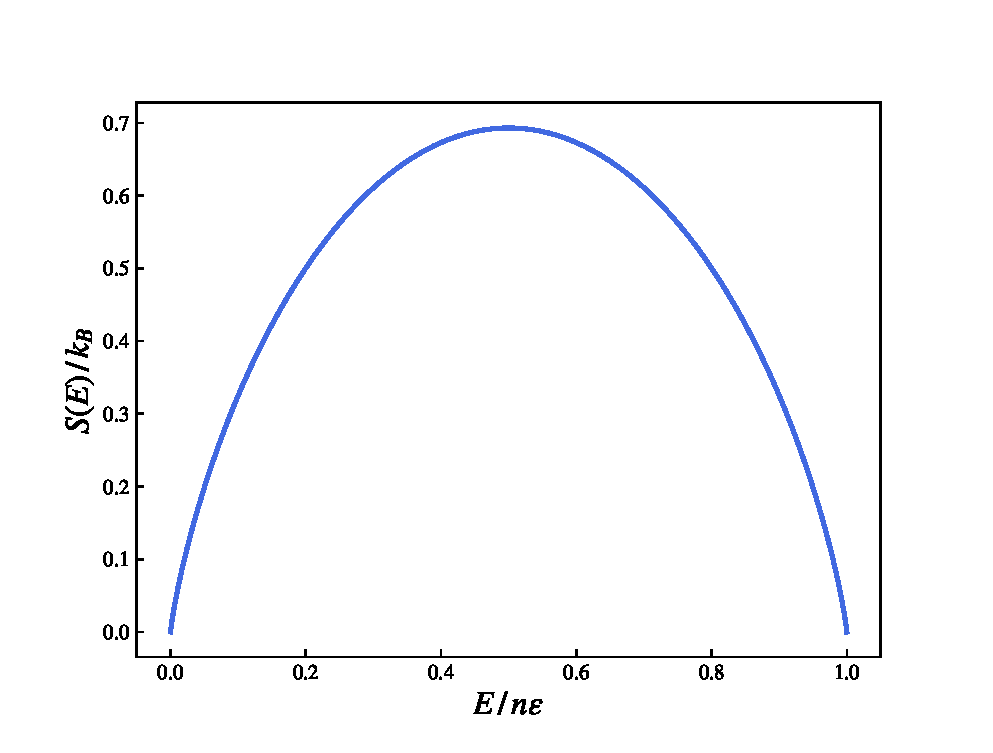
\includegraphics[scale=0.65]{images/entropy_TLS.eps}
    \caption{Entropy of a TLS as a function of the energy.}
    \label{fig:TLS_entropy_E}
\end{figure}
This insight can be formalized into \emph{Ramsey's criteria}.
\newpage
\section{Ramsey's criteria}
Ramsey \cite{Ramsey} provided 3 conditions under which a thermodynamic system exhibits negative temperatures
\begin{enumerate}
    \item \emph{The various elements of the thermodynamic system under analysis must be at equilibrium with each other}. \\
    This condition must be verified in order to define a temperature for the whole system.
    \item \emph{There must be an upper bound on the energy of the system} \\
    In fact it is known from statistical mechanics that the probability (or probability density) for the system to be in a state of energy $E$ is 
    \begin{equation}
        p(E) \propto e^{-\beta E}
        \label{eq:probability_ramsey}
    \end{equation}
    where $\beta = 1/k_BT$. If negative temperatures are admitted by the system and the latter does not admit an upper bound on the energy, the exponential factor in equation \ref{eq:probability_ramsey}
    becomes infinitely large for increasing energy. This means that if the system admits negative temperature, the higher the energy, the higher the probability of the system to be in that state. The most probable state 
    would then be the one at infinite energy making the other states negligible in probability. Clearly, an infinite amount of energy cannot be put into the system, meaning that such a system cannot exist.
    \item \emph{The thermodynamic system under analysis must be thermally isolated from other systems that do not satisfy the above conditions}. \\
    In good approximation one can think that the time required to reach equilibrium among the elements of the system is small compared to the time of interaction
    between the system and the environment or another system.
\end{enumerate}
The above conditions are all satisfied by the TLS described above. Indeed it admits negative temperatures. \\
\chapter{The experiment by Purcell and Pound}
\label{ch:PandP}

CONTROLLARE PARALLELO O ANTIPARALLELO

The existence of negative absolute temperatures was first predicted by Lars Onsager in 1949 \cite{Onsager} in the context of 2D confined turbulence vortices. \\
The confinement of the vortices caused the phase space of the system to be bounded and Onsager showed that this results in a peak of the entropy as a function of the energy, in accordance
to what stated by the Ramsey's criterion. \\
The first experimental evidence of negative temperatures was the experiment carried by Purcell and Pound \cite{PandP} in 1951, who managed to bring the spins of a LiF crystal in a negative absolute temperatures 
state for several minutes.
In this section I want to illustrate the experimental procedure followed by Purcell and Pound to realize such a state.\\

The experiment used a system of nuclear spins on a LiF crystal lattice immersed in a uniform magnetic field $\ve h$.
The energy of the system is given by the analogous of equation \ref{eq:Hamiltonian_lattice_spin}
\begin{equation*}
    E = - \ve h \cdot \ve M + \mathcal{H}_{ss} + \mathcal{H}_{sl}
\end{equation*}
where $\ve M$ is the magnetic moment vector $\ve M = g \frac{q}{2m} \, \ve S$, $\ve S$ is the spin and $g$ is the Landé factor. \\
As before we consider negligible the spin-spin interaction term but still considering it non-zero since it is fundamental for keeping the system in internal equilibrium \cite{main_article}. \\
The spin-lattice interaction is characterized by the typical relaxation time $\tau_{L}$ which was found to be around 5 minutes for the considered system. For times much smaller than $\tau_L$, 
the system can be considered as in a transient equilibrium, and the particle's states distribution defines a spin temperature according to equation \ref{eq:spin_temperature}. This temperature is precisely the one
that was deduced to be negative. The effective energy for the system for the experiment was then 
\begin{equation}
    E \approx - \ve h \cdot \ve M
    \label{eq:energy_PandP}
\end{equation}\\
Initially the system was brought into equilibrium aligning all the spins with the magnetic field in either a parallel or antiparallel way: for positive temperatures, for what said in chapter \ref{ch:TLS}, we expect the majority of the spins to be parallel causing the energy given by 
equation \ref{eq:energy_PandP} to be negative. \\
Then, suddently, the magnetic field is switched in direction, causing the majority of the spins to be antiparallel to the magnetic field, hence giving raise to a positive energy. This state is characterized by a negative spin temperature.
Figure \ref{fig:PandP_switch} illustrates the effect of the magnetic field making use of the entropy-energyrelation given by equation \ref{eq:entropy_E_TLS}.
\begin{figure}
    \centering 
    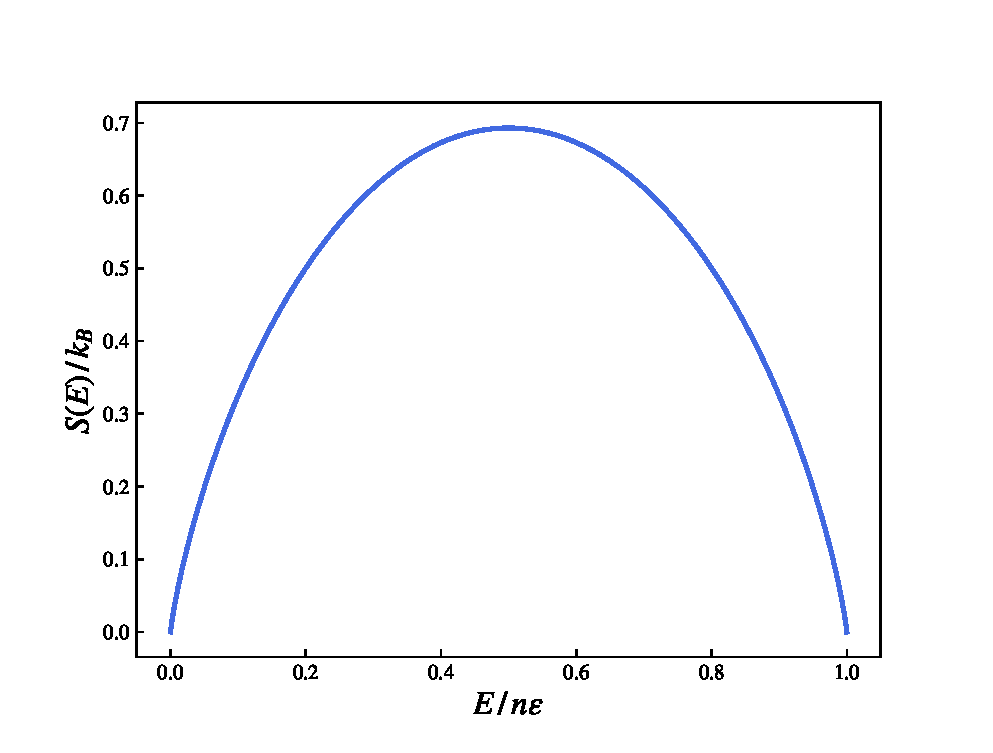
\includegraphics[scale=0.5]{./images/entropy_TLS}
    \caption{}
    \label{fig:PandP_switch}
\end{figure}
\begin{figure}[htbp]
    \centering 
    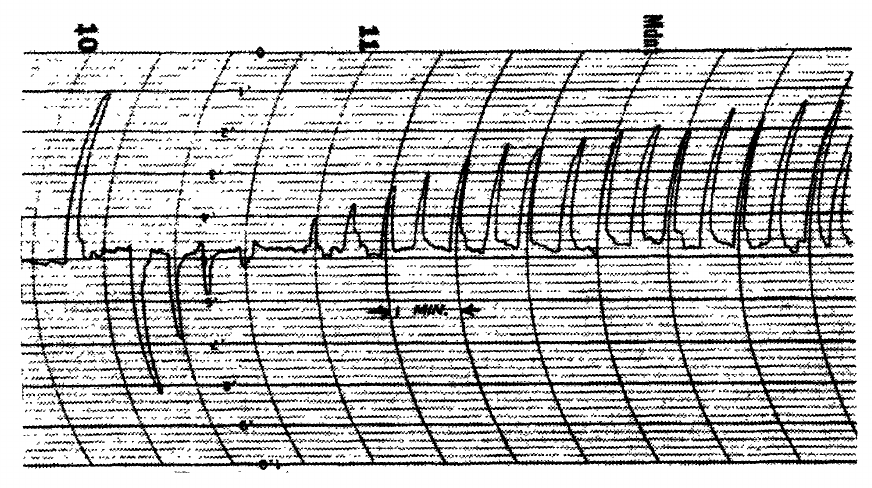
\includegraphics[scale=0.5]{./images/PurcellPound.png}
    \caption{The plot (adapted from \cite{PandP}) reports the record of the nuclear magnetization during the experiment. The first peak denotes
    the initial equilibrium state in which the spins are aligned with the magnetic field in the lowest energy state. As the magnetic field is istantaneously reversed,
    the spins remained aligned in the opposite direction of the field, remaining in the highest enery state and causing the second (negative) peak. After a relaxation time
    $\tau_L$ the spin system returns in equilibrium in the lowest energy state.}
    \label{fig:PandP}
\end{figure}
\chapter{Definition of Entropy}
\label{ch:entropy}
The temperature definition via
\begin{equation*}
    \frac{1}{T} = \frac{\partial S(E)}{\partial E}
\end{equation*}
is strictly dependent on the definition of the entropy and the existence of negative temperatures is mainly a consequence of this definition. 
It was already discussed in chapter \ref{ch:temperature} why it is legitimate to define the temperature as the derivative of the entropy with respect to the energy. The purpose of this section, on the other side,
is to discuss the definition of the entropy with particular regards to the definitions given by Gibbs and Boltzmann. since they have direct consequences on the existence of negative temperatures. \\
After a brief introduction over the two perspectives, which would require an entire thesis themselves to be deeply developed, the focus of the discussion will be on the comparison between the two definitions with particular emphasis on the direct consequences on the negative temperatures.

\section{Boltzmann's framework}
The conceptual basis for the Boltzmann's approach to statistical mechanics presented in Boltzmann's paper (1877b) relies on the attempt to explain the Second Law of thermodynamics via probability calculus. \\
To introduce the idea let us consider a system of $N$ particles and let us work in a $6N$ dimensional phase space with coordinates $q_1,...,q_{3N}, p_1, ... p_{3N}$ and let us consider also the $\mu$-space associated to each particle in the system, i.e. the phase space in which each single particle moves. \\
Let us parition each $\mu$-space into $m$ disjoint rectangular cells of volume $\Delta\omega$ so that $\mu = \omega_1 \cup ... \cup \omega_m$ and each cell $\omega_i$ is charaterized by an energy value $\epsilon_i$. Once specifying the mechanical state of the system, a point $x \in \Gamma$, one can 
associate a collection of $N$ points in the $\mu$-spaces, one for each particle (they are the same for each particle). For each $x$, also called \emph{microstate} of the system, one can define a \emph{macrostate} for the system by specifying the number of particles $n_i$ included in each cell $\omega_i$ in the $\mu$-space. 
Formally $Z = (n_1, ... , n_m)$ where $n_i$ is the number of particles in the cell $\omega_i \subset \mu$. \\
By this definition it is clear that more than one microstate can describe the same macrostate of the system. For each macrostate $Z_0$ the corresponding phase space volume, that is the set of corresponding microstates, is 
\begin{equation*}
    \Gamma_{Z_0} \equiv \{x \in \Gamma : Z(x) = Z_0\}
\end{equation*}
The Boltzmann's entropy of a system in a macrostate $Z$ is then defined as
\begin{equation}
    S = k_B \ln\left( \text{Vol}(\Gamma_Z)\right)
    \label{eq:Boltzmann_entropy}
\end{equation}

\section{Gibbs' framework}
Gibbs' approach to statistical mechanics is based on the idea of a statistical ensemble. To introduce this concept
let us work again in a phase space $\Gamma$ and describe the system via $3N$ canonical coordinates, so that $\Gamma$ is a $6N$ dimensional space. A point in $\Gamma$ denotes
a precise configuration of the system and it is referred to as a \emph{representative point}. \\
A given macroscopic configuration for the system can correspond to multiple microscopic configurations of the system, that is multiple points in the $\Gamma$ space might correspond to the same macroscopic state. \\
In other words, when specifying a precise macroscopic configuration, we are not referring to one system, but rather to a collection of systems which we call an \emph{ensemble}. \\
An ensemble is conveniently described my means of a \emph{density function} $\rho(q, p ,t)$ such that $\rho(q, p, t) d^{3N}qd^{3N}p$ is the number of representative points in a phase space volume $d^{3N}qd^{3N}p$. \\
Given the value of $\rho$ at time $t=0$, the evolution of the function is completely determined by means of the Hamilton equation 
\begin{gather*}
    \frac{dp_i}{dt} = -\frac{\partial \mathcal H}{\partial q_i} \\
    \frac{dq_i}{dt} = \frac{\partial \mathcal H}{\partial p_i}
\end{gather*}
More precisely the evolution of $\rho$ is determined by the \emph{Liouville's theorem} which states that
\begin{equation}
    \frac{\partial \rho}{\partial t} + \sum_{i=1}^{3N} \left(\frac{\partial \rho}{\partial p_i}\dot p_i + \frac{\partial \rho}{\partial q_i} \dot q_i\right) = 0
\end{equation}
or 
\begin{equation*}
    \frac{\partial \rho}{\partial t} = \left\{H, \rho\right\}
\end{equation*}
ADD PROOF OF THE Liouville's theorem. \\
\vspace{10pt}
In developing his theory, Gibbs' main goal was to produce a rational fundation for thermodynamics. Hence, Gibbs's work was guided by analogies between his theory and thermodynamics. \\
In his book \cite{gibbs_2010} Gibbs derived a relation in the canonical ensemble that is
\begin{equation}
    d\left\langle H \right\rangle = \theta d\sigma - \sum_i \left\langle A \right\rangle da_i
    \label{eq:fundamentaleq_Gibbs}
\end{equation}
which is formally analogue to the fundamental equation of thermodynamics
\begin{equation*}
    dU = TdS + \sum_i F_i da_i
\end{equation*}
where $\left\langle H \right\rangle$ in equation \ref{eq:fundamentaleq_Gibbs} denotes the expectation value of the hamiltonian in the canonical ensemble.
The analogy suggests that $\theta$, the so called \emph{modulus of the ensemble}, can be identifies as the temperature of the system and  and $\sigma$, defined as
\begin{equation*}
    \sigma[p_{\theta}] = - \int p_{\theta}(x) \ln \rho_{\theta}(x) \, dx
\end{equation*}
can be identified as the entropy of the system, namely the \emph{Gibbs entropy}. \\
One important point to note is that in the Gibbs' entropy is not a function on the phase space but rather a functional on the ensemble density $\rho_{\theta}$. This implies that there is no function $\chi$ on the phase space such that 
\begin{equation*}
    \left\langle \chi \right\rangle_{\theta} = \sigma[\rho_{\theta}] \quad \forall \theta
\end{equation*}
The next step is to understand whether an equation such \ref{eq:fundamentaleq_Gibbs} can be obtained in the microcanonical ensemble. Gibbs proposed (see \cite{gibbs_2010} page 124-128, 169,171) the following definitions
\begin{gather*}
    T \quad \longleftrightarrow \quad \left(\frac{\partial \ln \Omega(E)}{\partial E}\right)^{-1} \\
    S \quad \longleftrightarrow \quad \ln \Omega(E)
\end{gather*}
where 
\begin{equation}
    \Omega(E) \equiv \int_{H(x) \leq E} \, dx
    \label{eq:Omega_E}
\end{equation}
is called \emph{integrated density of states}. 

\section{Consistent thermodynamics forbids negative temperatures}
The difference between the Gibbs entropy \footnote{the Boltzmann's constant is added for dimensional arguments}
\begin{equation}
    S_G = k_B \ln \Omega(E)
    \label{eq:gibbs_entropy_formula}
\end{equation}  
and the Boltzmann's entropy 
\begin{equation}
    S_B = k_B \ln \omega(E)
    \label{eq:Boltzmann_entropy_formula}
\end{equation}
has a direct and important consequence on the existence of negative temperatures. Indeed it is easy to see that the integrated density of states defined in equation 
\ref{eq:Omega_E}, that is the number of states whose energy is less than or equal to $E$, is a monotonically increasing function of the energy, hence the temperature is always positive. On the other side,
the density of states $\omega(E)$ that enters in the Boltzmann's entropy denotes the number of states in the range $(E, E+dE)$ and there is no reason to believe that is a monotonically increasing function of the energy. In fact we have already seen
that in the case of a non interacting two level system the Boltmann's entropy leads to negative temperatures. \\
The choice of the correct microcanonical entropy is not a straightforward process since different definitions of entropy can be used untill they are able to reproduce the thermodynamics. \\
In 1991 Berdichevsky \textit{et al.} \cite{original_entropy} pointed out some arguments in favour of the Gibbs' entropy, which have then been developed by many authors. The main arguments were proposed by 
Dunkel and Hillbert in 2014 \cite{Dunkel_Hillbert} introducing the so called \emph{thermostatistical consistency condition}. \par 
\vspace{10pt} 
Let us suppose that the system is described by some control variables $\{E, V, A_i\}$ so that $S = S(E, V, A_i)$. By differentiating $S$ with respect to the control variables 
\begin{equation*}
    \begin{aligned}
        \mathrm{d} S &=\left(\frac{\partial S}{\partial E}\right) \mathrm{d} E+\left(\frac{\partial S}{\partial V}\right) \mathrm{d} V+\sum_{i}\left(\frac{\partial S}{\partial A_{i}}\right) \mathrm{d} A_{i} \\
        & \equiv \frac{1}{T} \mathrm{~d} E+\frac{p}{T} \mathrm{~d} V+\sum_{i} \frac{a_{i}}{T} \mathrm{~d} A_{i}
        \end{aligned}
\end{equation*}
If one now considers an isoentropic process for which only energy and one control variable are allowed to change, one gets that
\begin{equation}
    T\left(\frac{\partial S}{\partial A_{\mu}}\right)_{E}=-\left(\frac{\partial E}{\partial A_{\mu}}\right)_{S}=-\left\langle\frac{\partial H}{\partial A_{\mu}}\right\rangle
    \label{eq:cond1}
\end{equation}
Now, since
\begin{equation*}
    \begin{array}{l}
        T_{\mathrm{B}}(E, V, A)=\left(\frac{\partial S_{\mathrm{B}}}{\partial E}\right)^{-1}=\frac{1}{k_{\mathrm{B}}} \frac{\omega}{\omega^{\prime}}=\frac{1}{k_{\mathrm{B}}} \frac{\Omega^{\prime}}{\Omega^{\prime \prime}} \\
        T_{\mathrm{G}}(E, V, A)=\left(\frac{\partial S_{\mathrm{G}}}{\partial E}\right)^{-1}=\frac{1}{k_{\mathrm{B}}} \frac{\Omega}{\Omega^{\prime}}=\frac{1}{k_{\mathrm{B}}} \frac{\Omega}{\omega}
        \end{array}
\end{equation*}
we expect that if one of the two definitions of the entropy satisfies the condition \ref{eq:cond1}, the other one does not. \\
The Gibbs entropy satisfies the condition
\begin{equation*}\begin{aligned}
    T_{G}\left(\frac{\partial S_{G}}{\partial A_{\mu}}\right) &=\left(\frac{\partial S_{G}}{\partial E}\right)^{-1}\left(\frac{\partial S_{G}}{\partial A_{\mu}}\right)=\frac{1}{\omega} \frac{\partial}{\partial A_{\mu}} \operatorname{Tr}[\theta(E-\mathcal{H})] \\
    &=\frac{1}{\omega} \operatorname{Tr}\left[\frac{\partial \theta(E-\mathcal{H})}{\partial A_{\mu}}\right]=-\frac{1}{\omega} \operatorname{Tr}\left[\delta(E-\mathcal{H}) \frac{\partial \mathcal{H}}{\partial A_{\mu}}\right] \\
    &=-\operatorname{Tr}\left[\frac{\delta(E-\mathcal{H})}{\omega} \frac{\partial \mathcal{H}}{\partial A_{\mu}}\right]=-\operatorname{Tr}\left[\rho \frac{\partial \mathcal{H}}{\partial A_{\mu}}\right]=-\left\langle\frac{\partial \mathcal{H}}{\partial A_{\mu}}\right\rangle
\end{aligned}\end{equation*}
so the Boltzmann's cannot
\chapter{Simulating a system at negative temperature}

\section{The Ising Model}
Brief introduction to the Ising Model

\section{Single system at negative temperature}

\section{Two systems into contact}
Two systems are prepared at temperature $T_1$ and $T_2$. The spin configurations are obtained after $10^4$ Monte Carlo cycles in the canonical ensemble. \\
After that, the two systems are put into contact forming a new system that can be threated as a microcanonical ensemble. The simulation of the latter was obtained with a 
demon Monte Carlo method with $10^6$ cycles.

\begin{figure}[h]
    \centering
    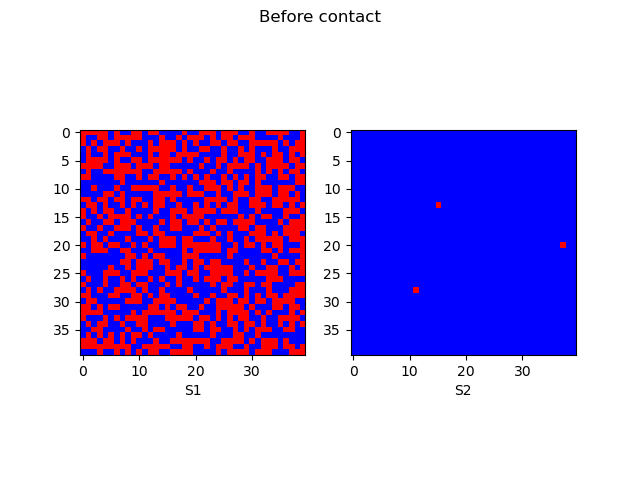
\includegraphics[scale=0.7]{./images/T1_T2_before.png}
    \caption{Before contact}{The red tiles indicate the \emph{up} state, while the blue tiles indicate the \emph{down} state. Before beeing put into contact
    the two systems are prepared respectively at temperature $k_B T_1 = -\infty \, (10^8)$ and $k_B T_2 = 0^+ \, (10^{-8})$}
    \label{fig:before}
\end{figure}

\begin{figure}[h]
    \centering
    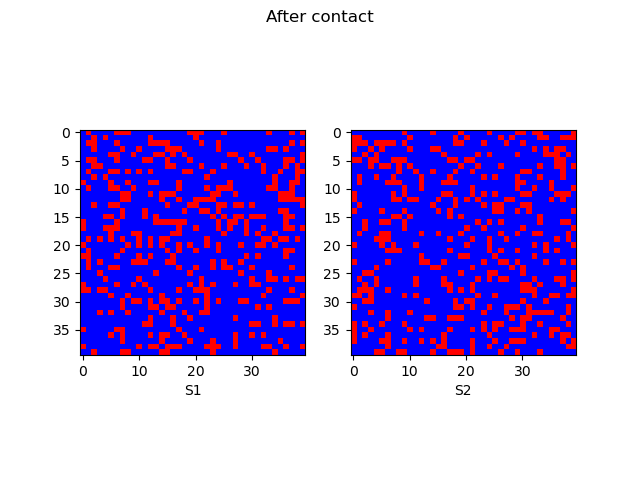
\includegraphics[scale=0.7]{./images/T1_T2_after.png}
    \caption{After contact}{The red tiles indicate the \emph{up} state, while the blue tiles indicate the \emph{down} state. The equilibrium temperature after putting the two systems into contact is in between the two values according to the hierarchy presented 
    at the end of chapter \ref{ch:temperature}. The system at negative temperature get cooled down changing some up states to down states, while the system at positive temperature
    gets heated changing some down states into up. The resuls is of course an approximately equal concentrarion of up/down in both systems.}
    \label{fig:after}
\end{figure}

\printbibliography
\nocite{*}

\end{document}

%%%%%%%%%%%%%%%%%%%%%%%%%%%%%%%%%%%%%%%%%%%%%%%%%%%%%%%%%%%%%%%%%%%%%%%%%%%%%%%
%                                                                             %
% *** END OF THIS BACHELOR THESIS PROJECT ***                                 %
%                                                                             %
%%%%%%%%%%%%%%%%%%%%%%%%%%%%%%%%%%%%%%%%%%%%%%%%%%%%%%%%%%%%%%%%%%%%%%%%%%%%%%%